\section{Results}
\label{sec:results}

\subsection{The reference spectrum and the meaning of a free-shift improvement}

In the six-transition ESPRESSO reference fit, the restricted conventional model has 147 parameters and the alternative has 152. Both use the same 2931 retained pixels. The selected diagonal-error endpoints give $Q_0=2305.49$ and $Q_1=2253.78$, an improvement of $51.71$ for five relative shifts. The 2382 and 2600 shifts are approximately $-118$ and $-109\,\mathrm{m\,s^{-1}}$ relative to 2374. Figure~\ref{fig:reference_profiles} shows the actual profiles and residuals. Several nuisance parameters lie near their bounds, and different starts find different local solutions. The improvement therefore establishes a conditional preference within this particular comparison; it is not assigned a discovery significance or interpreted as a measurement of $\Delta\alpha/\alpha$.

The alternative supplied expected-fluctuation error array increases the diagonal-error improvement to $67.92$, with $Q_0=2801.71$ and $Q_1=2733.79$. Thus the recorded controls do not uniformly weaken the preference. This noise-amplitude change is distinct from the continuum-derived correlation-shape test below. The complete saved control grid includes both stronger and weaker conditional improvements.

\begin{figure}[htbp]
\centering

\includegraphics[width=.94\textwidth,height=.68\textheight,keepaspectratio]{espresso_conventional_null.pdf}
\caption{The six observed Fe\,II transitions in the reference ESPRESSO interval, with shared-gas fits and standardized residuals. The conventional and free-relative-shift models have the same gas and continuum freedoms. A better fit after adding shifts is a diagnostic of the specified model, not an identification of the physical origin of the discrepancy.}
\label{fig:reference_profiles}
\end{figure}

\subsection{Correlated noise, core exclusions and retained information}

Twenty-five non-overlapping continuum intervals contain 13,750 pixels. After local continuum removal, their lag-one correlation is $0.3726$. We use the measured correlation shape with a finite taper, retaining the supplied error amplitude. This is a covariance model transferred from continuum diagnostics, not a measured full covariance for the absorption spectrum. The generalized least-squares comparison reduces the five-shift improvement to $29.24$. The nonlinear fit re-optimizes gas and continuum parameters under the changed weights; it is not a rescaling of the diagonal-error result.

The joint controls apply the frozen strong-line exclusions and the same tapered correlation model simultaneously. The milder mask leaves 2692 pixels and gives an improvement of $23.69$; the padded wider mask leaves 2473 pixels and gives $6.70$. Table~\ref{tab:control_comparisons} lists within-row comparisons. The relevant hypotheses use identical pixels and covariance within each row, whereas objective differences across rows do not have a common likelihood-ratio interpretation.

\begin{table}[htbp]
\centering
\caption{Conditional reference-spectrum comparisons. $k_0$ counts conventional-model parameters; each alternative adds five shifts. GLS retains the supplied variance amplitude. All rows describe selected bounded local endpoints, with no global-optimum certification.}
\label{tab:control_comparisons}
\small
\begin{tabular}{lrrrr}
\toprule
Selection and gas architecture & Pixels & $k_0$ & $Q_0$ & $\Delta Q$ \\
\midrule
Statistical errors, diagonal, 45 components & 2931 & 147 & 2305.49 & 51.71 \\
Expected fluctuations, diagonal, 45 components & 2931 & 147 & 2801.71 & 67.92 \\
Full pixels, GLS, 45 components & 2931 & 147 & 2231.33 & 29.24 \\
Joint $F<0.1$ mask + GLS & 2692 & 147 & 1931.90 & 23.69 \\
Joint padded $F<0.3$ mask + GLS & 2473 & 147 & 1684.36 & 6.70 \\
Full pixels, GLS, 40 components & 2931 & 132 & 2255.16 & 18.87 \\
\bottomrule
\end{tabular}

\end{table}

Masking changes both model sensitivity and the available information. At the same fixed diagonal-noise conventional endpoint, we project the five shift derivatives against the gas and continuum derivatives under each GLS selection. For the specified direction in which 2382 and 2600 each move by $100\,\mathrm{m\,s^{-1}}$ and the other three shifts remain zero, the milder and wider masks retain $70.5\%$ and $16.0\%$ of the unmasked local information (Fig.~\ref{fig:core_information}). The direction was chosen to illustrate the previously observed strong-line pattern; it is not a prediction independent of these data. The calculation uses an unconstrained tangent space despite active parameter bounds. It follows that a smaller improvement after core removal cannot by itself establish that saturation caused the original shifts. Conversely, this calculation does not establish that information loss accounts for the full reduction.

\begin{figure}[htbp]
\centering

\includegraphics[width=.98\textwidth]{joint_controls_information.pdf}
\caption{Actual nonlinear objective improvements (left) and a separate local sensitivity calculation (right). The latter describes one specified coherent strong-line direction after projection over common nuisance parameters, not the marginal information for five free shifts. Diagonal and GLS fits within each mask are actual re-fits; different masks retain different information.}
\label{fig:core_information}
\end{figure}

\subsection{Gas architecture and optimization dependence}

The fixed merging rule yields 40 components from the 45 published starting components. On the full set of 2931 pixels, the 132-parameter conventional GLS model gives $Q_0=2255.16$ and the 137-parameter alternative gives $Q_1=2236.29$, an improvement of $18.87$. The 2382 and 2600 shifts become approximately $-89$ and $-80\,\mathrm{m\,s^{-1}}$, each changing by about $22\,\mathrm{m\,s^{-1}}$ from the 45-component GLS values. Two alternative-model starts terminate at objectives differing by $12.95$. Thus architecture and initialization affect the result even though this particular reduced architecture does not remove the conditional shift preference. Because the merged starting centres also define the shifted parameter-bound centres, this is an architecture-and-bounds sensitivity test, not a nested determination of the correct number of gas clouds.

The independent UVES photons from the same absorber provide an additional, explicitly limited check. Three Fe\,II lines contain 511 usable pixels. Using the recommended expected-fluctuation errors, we continue fits with Gaussian-width scales bounded by $[0.65,1.25]$ and $[0.5,1.4]$ times the catalogue value. Four 1800-evaluation continuations and one 400-evaluation conventional cross-start all reach their evaluation caps and fail the specified first-order stationarity criteria. The lowest saved conventional parameter vector is feasible in both domains. Relative to that vector, the finite objective reductions are $9.75$ and $10.08$ for two shifts; widening the instrumental-width bounds changes the strong-line offsets by only $4$--$5\,\mathrm{m\,s^{-1}}$. These nonstationary endpoint differences receive no calibrated significance. The archived product records wavelength shift and slope corrections, whose equivalence to a dedicated precision-analysis product has not been established. Independent photons therefore do not supply an independent model or a completed physical confirmation.

\subsection{Native-exposure and same-transition order tests}
\label{sec:order_results}
The fixed-template estimator applied to the 17 individual exposures gives pooled 2382 and 2600 shifts relative to 2374 of $-41.9\pm16.4$ and $-45.5\pm15.0\,\mathrm{m\,s^{-1}}$. Applying the same estimator to the combined spectrum gives $-42.8$ and $-39.6\,\mathrm{m\,s^{-1}}$. These are compatible representations of the same observations, not independent confirmations. They are also different estimators from the joint fits in which all gas parameters are re-optimized. The original exposure analysis finds no clear excess heterogeneity or difference between the nine 2018 and eight later exposures under its conditional covariance model.

The same-transition comparison removes the atomic reference entirely. In the initial per-exposure calculation, the lower-index minus upper-index order contrast is $-60.25\pm16.72\,\mathrm{m\,s^{-1}}$ for 2600, compared with $-10.53\pm21.87\,\mathrm{m\,s^{-1}}$ for 2382. The two traces separately retain the 2600 pattern, and deleting any single exposure gives means between approximately $-70.1$ and $-52.0\,\mathrm{m\,s^{-1}}$. The diagnostic is therefore not dominated by one exposure or one trace. The barycentric velocity and detector position are nearly collinear in these observations, preventing their simple regressions from locating the mechanism.

We next fit all exposures jointly with the Gaussian and centred positive-mixture response families defined in Sec.~\ref{sec:methods}. Each family has matched comparisons with and without a single order-contrast parameter. This jointly shared response estimator is slightly different from independently fitting each exposure. The completed comparisons are shown in Table~\ref{tab:order_models} and Fig.~\ref{fig:order_models}.

\begin{table}[htbp]
\centering
\caption{Native-pixel order-response controls. The order contrast is the lower-index minus higher-index order velocity for the same transition, distinct from the cross-transition descriptor $D$. G denotes the Gaussian response; A denotes the specified positive, zero-centroid asymmetric family. Subscripts indicate whether a free order contrast is added. Errors are local, conditional on the fixed gas template and diagonal extraction errors. $\Delta Q$ compares models within the indicated response family, not different transitions.}
\label{tab:order_models}
\small
\begin{tabular}{llrrr}
\toprule
Transition & Response & $Q$ & Order contrast ($\mathrm{m\,s^{-1}}$) & $\Delta Q$ \\
\midrule
2600 & G$_0$ & 41636.411 & 0 (fixed) & --- \\
2600 & G$_1$ & 41622.198 & $-62.75\pm16.66$ & 14.212 \\
2600 & A$_0$ & 41630.900 & 0 (fixed) & --- \\
2600 & A$_1$ & 41620.042 & $-58.64\pm18.65$ & 10.858 \\
2382 & G$_0$ & 39994.136 & 0 (fixed) & --- \\
2382 & G$_1$ & 39993.889 & $-11.03\pm22.18$ & 0.247 \\
2382 & A$_0$ & 39994.062 & 0 (fixed) & --- \\
2382 & A$_1$ & 39993.787 & $-13.48\pm26.35$ & 0.275 \\
\bottomrule
\end{tabular}
\end{table}

The specified asymmetric family does not remove the 2600 contrast. Relative to G$_1$, two shape parameters reduce $Q$ by only 2.16. Forcing a zero order contrast in A$_0$ drives one shape parameter to its bound. The asymmetric fit has nominal $Q/(N-k)\simeq1.34$ for 2600 and 1.29 for 2382, so even the extended response does not supply an adequate complete noise-and-profile description. Conditional objective profiles explicitly re-optimize the remaining parameters at 13 order offsets from $-120$ to $+120\,\mathrm{m\,s^{-1}}$. They confirm the local displacement preference while exposing shape boundaries; they do not supply a calibrated discovery probability. The shape parameterization is not generally twice continuously differentiable at its Gaussian limit, providing another reason to avoid an automatic Wilks interpretation.

\begin{figure}[htbp]
\centering
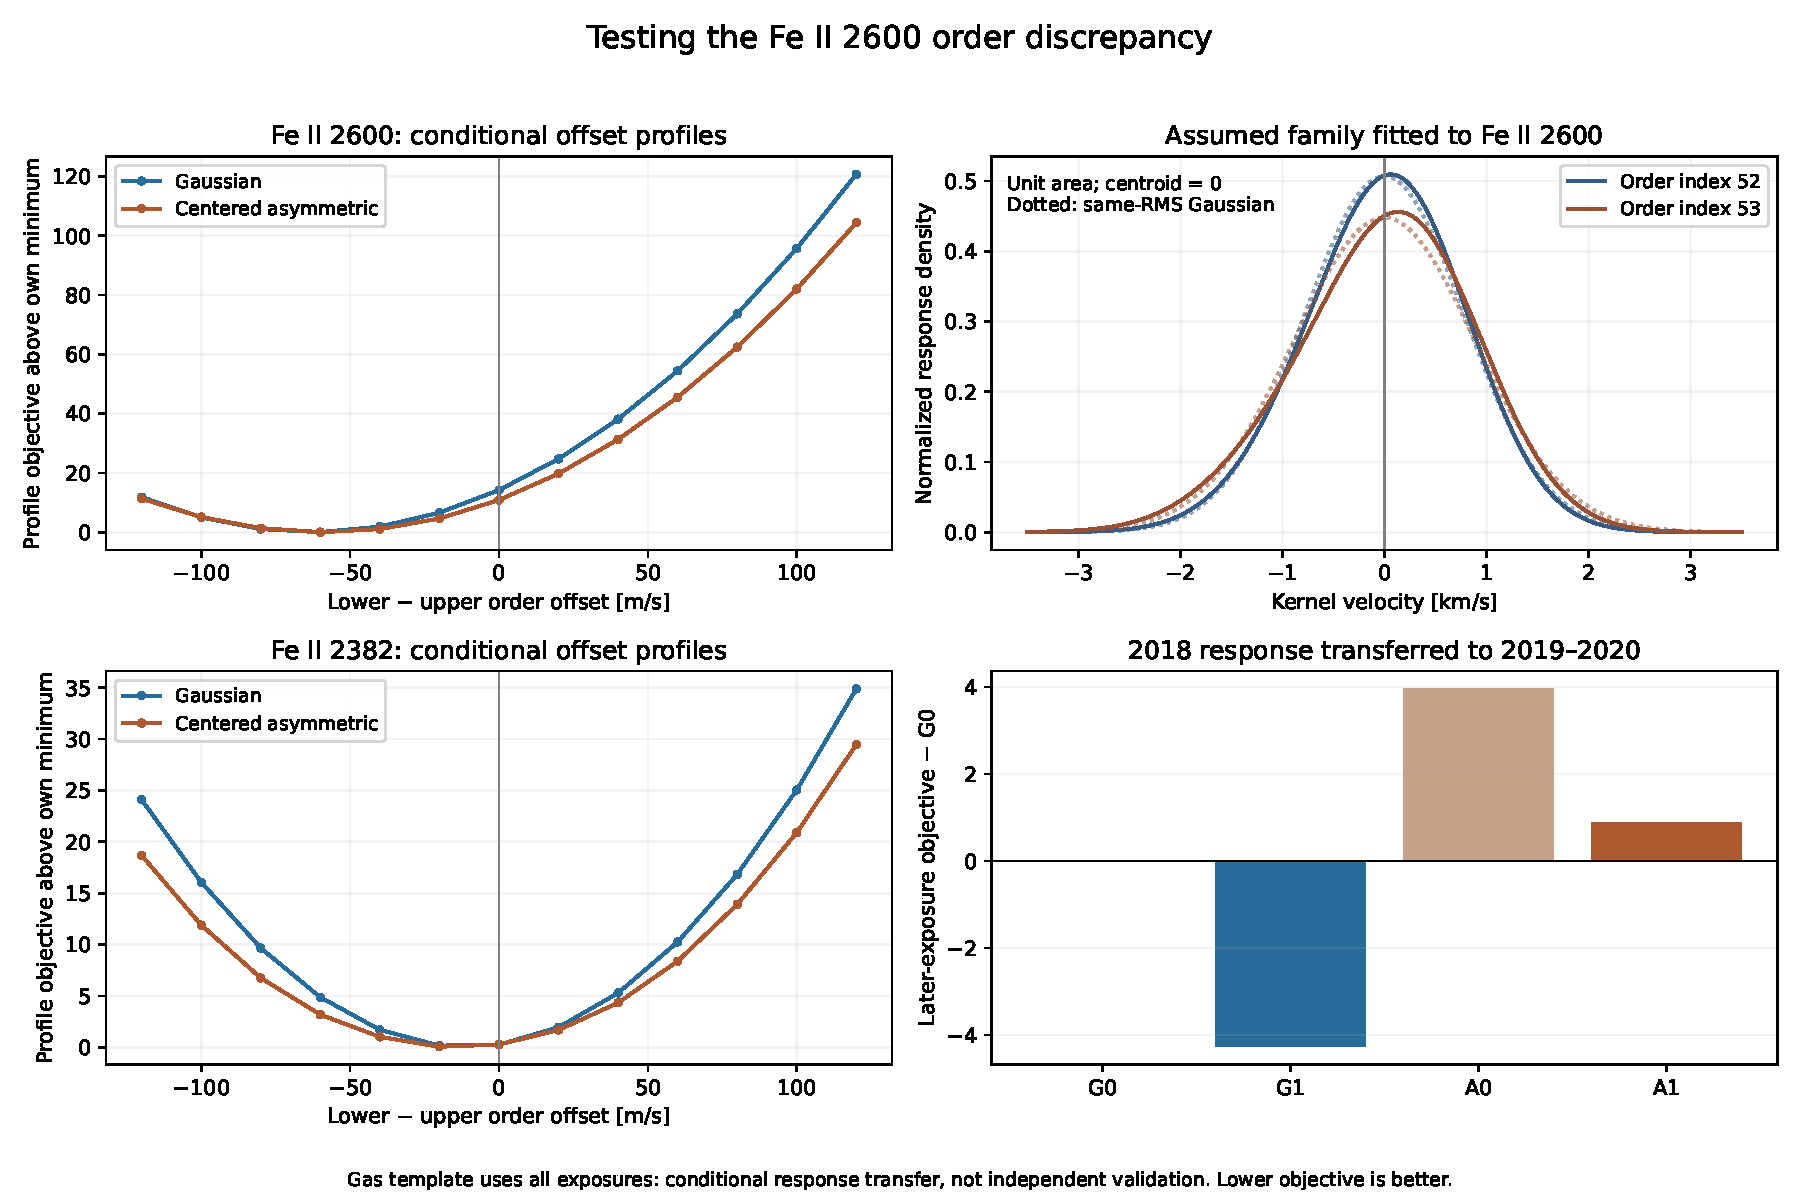
\includegraphics[width=.99\textwidth]{../experiments/highz_feasibility_2026-09-20/results/order_response/order_response_models.pdf}
\caption{Tests of the specified centred response family using actual native pixels. The order-contrast profiles re-optimize nuisance parameters at fixed contrast. The response-family illustration does not represent an independently measured LSF. The later-exposure comparison transfers response parameters learned from 2018, while the gas template remains shared with the full data set; it is therefore a conditional transfer diagnostic.}
\label{fig:order_models}
\end{figure}

In that transfer diagnostic, the Gaussian-plus-contrast model improves the later-exposure objective by 4.27 relative to the Gaussian zero-contrast model. The asymmetric-plus-contrast model is worse than Gaussian-plus-contrast by 5.15. This does not establish a transferable benefit from the extra shape parameters. An instrumental response that genuinely changes across epochs remains possible, and the shared combined-spectrum gas template prevents a fully independent predictive interpretation.

The orders also have different sampling, masks and signal-to-noise weights. A further mask control retains a native pixel only when its entire wavelength bin is covered by the other order's originally valid bins; selection uses wavelength geometry and existing quality masks, not new residual clipping. It retains 62,154 of 62,404 relevant pixels. The resulting 2600 contrast is $-58.65\pm16.75\,\mathrm{m\,s^{-1}}$, and the 2382 contrast is $-15.45\pm21.98\,\mathrm{m\,s^{-1}}$. Missing coverage alone, under this particular control, does not remove the pattern. Sampling and weighting still differ, so a shared imperfect gas template could produce different apparent velocities without a pure calibration offset.

Independent calibration remains unresolved. The released science headers identify the same \texttt{espdr/2.2.3}, SINGLEHR, $2\times1$ mode and LFC/FP wavelength products. For two representative science frames, current default archive master associations instead return THAR/FP wavelength products. Their association status does not establish reproduction of the released LFC solution. We locate historical raw LFC candidates and preserve their headers and association trees, but the checked public links do not yield uniquely matched historical LFC masters or independently measured response kernels. The 2024 response study used 2023 calibration data \citep{Schmidt2024LSF}; its method motivates this investigation, while its measured kernels cannot simply be assigned to the 2018--2020 science exposures. The bounded controls therefore locate a robust conditional order inconsistency without identifying its unique cause or measuring an intrinsic atomic change.


\subsection{The complete screened absorber sample}
\label{sec:archive_results}
The catalogue screen initially retains 36 absorbers in 32 spectra. Extending the atmospheric exclusion to broad water bands leaves seven metadata candidates; actual-pixel inspection leaves six multiplet candidates. All six are retained in the physical-model accounting in Table~\ref{tab:archive_six}, including models that remain inadequate. These are selected DLA sightlines, not a complete or statistically representative sample of metal absorbers.

For the four newly modelled candidates, an exploratory adequacy gate requires $Q_0/(N-k_0)\leq1.5$, every line's $Q/N_{\rm line}\leq1.8$, and successful optimizer termination. The thresholds are working diagnostics under the stated diagonal errors, not calibrated goodness-of-fit probabilities. Component grids, windows and visible contamination warnings were recorded before the new relative-shift fits, with documented null-model grid extensions. Because an $H_0$ gate could also reject a genuinely shifted system, we additionally perform bounded free-shift and crossed-null diagnostics for both gate failures on their unchanged primary pixels. They remain inadequate, and we do not promote them to precision measurements or use the gate to infer population-level constancy.

\begin{table}[htbp]
\centering
\caption{Latest matched conventional/free-shift comparisons for all six archive candidates. $n_g$ is the shared gas-component count and $k_\delta$ the number of additional shifts. Values use native pixels and diagonal expected-fluctuation errors. ``Conditional'' permits a model-specific displacement diagnostic, not a calibrated atomic-frequency measurement. ``Inadequate'' retains the post-screen diagnostic comparison on the original primary data. All pairs retain model and optimization limitations described in the text.}
\label{tab:archive_six}
\small
\begingroup
\setlength{\tabcolsep}{4pt}
\begin{tabular}{lrrrrrl}
\toprule
Target ($z$) & Pixels & $n_g$ & $Q_0$ & $\Delta Q$ & $k_\delta$ & Status \\
\midrule
J232128$-$105122 (1.629) & 130 & 3 & 75.16 & 6.16 & 4 & Conditional \\
J225719$-$100104 (1.836) & 504 & 30 & 421.25 & 13.53 & 2 & Conditional \\
J053007$-$250329 (2.141) & 480 & 16 & 482.30 & 4.18 & 3 & Conditional \\
J233156$-$090802 (2.143) & 1176 & 26 & 1672.84 & 5.54 & 2 & Inadequate \\
J004131$-$493611 (2.248) & 138 & 6 & 95.23 & 7.97 & 2 & Conditional \\
J064326$-$504112 (2.659) & 436 & 16 & 532.23 & 4.64 & 3 & Inadequate \\
\bottomrule
\end{tabular}
\endgroup

\end{table}

The initial two pilots now have actual nuisance-refitted profiles for $D=v_{2382}-v_{2374}$ (Fig.~\ref{fig:archive_pair}). For J232128$-$105122, the latest matched full-model comparison gives $Q_0=75.1589$, $Q_1=68.9988$ and $\Delta Q=6.1600$ for four added shifts. Its $D=-339.97\,\mathrm{m\,s^{-1}}$ has unconstrained local tangent error $179.58\,\mathrm{m\,s^{-1}}$; the connected profile has linearly interpolated $\Delta Q=1$ crossings between optimized grid points at $[-495.18,-187.88]\,\mathrm{m\,s^{-1}}$. Several zero-level parameters are bound-active. Neither the local error nor the profile contour includes calibration or gas-architecture uncertainty.

J004131$-$493611 illustrates why a stopped optimizer is not a certified solution. Profiling discovered a substantially lower nuisance basin than the earlier pair $(Q_0,Q_1)=(110.0357,104.5341)$. Restarting both full hypotheses fairly gives $(95.2285,87.2549)$, hence $\Delta Q=7.9735$ for two shifts. The revised $D=-120.11\,\mathrm{m\,s^{-1}}$ has local tangent error $399.41\,\mathrm{m\,s^{-1}}$, whereas the bounded connected $\Delta Q=1$ contour, linearly interpolated between optimized grid points, is $[-264.86,+39.96]\,\mathrm{m\,s^{-1}}$. Active gas-width, response-width and zero-level bounds may contribute to this discrepancy; nonlinearity and residual curvature have not been separately isolated. These are conditional objective contours, not coverage-calibrated confidence intervals. Fixing $D=0$ still lets 1608 move and therefore does not recover the full $H_0$.

\begin{figure}[htbp]
\centering
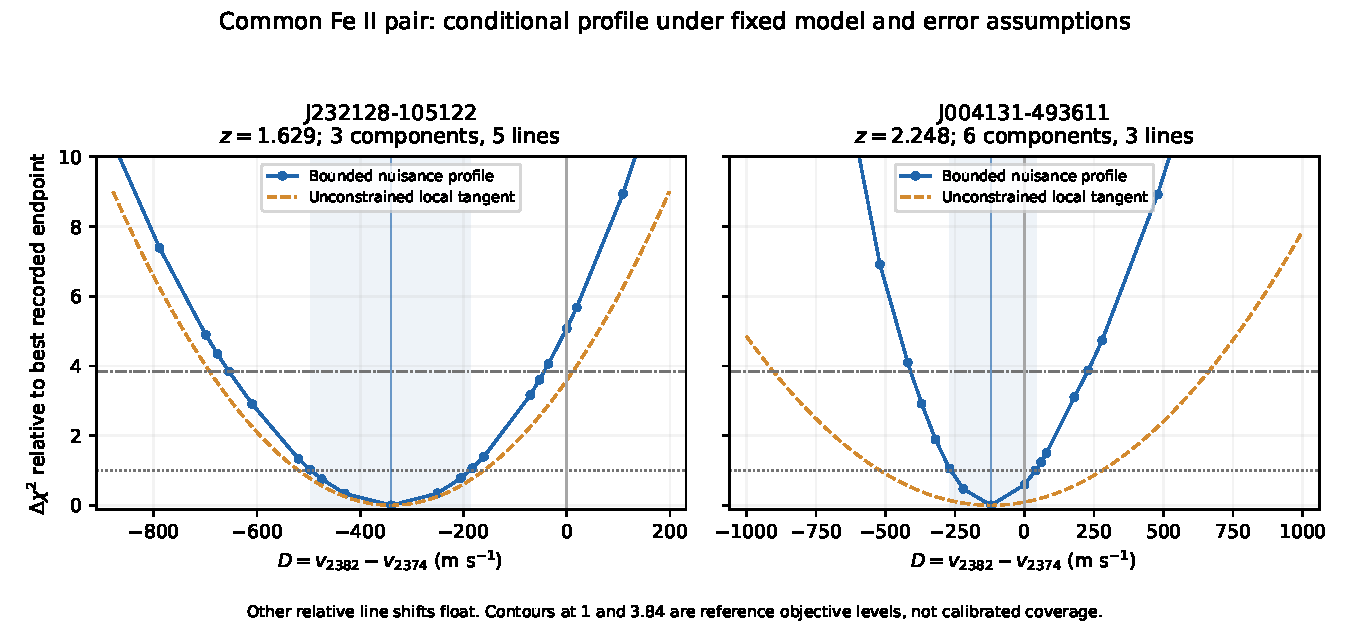
\includegraphics[width=.95\textwidth]{../experiments/highz_feasibility_2026-09-20/results/common_pair/common_pair_profiles.pdf}
\caption{Actual conditional profiles of the common 2382/2374 descriptor in the two initial pilots. Gas and other nuisance parameters, including the other relative line shifts, are refitted. Only endpoints in the final selected nuisance basins are connected; earlier inferior endpoints remain in the archive. Horizontal objective levels are descriptive. They do not calibrate systematic uncertainties, component selection or disconnected minima.}
\label{fig:archive_pair}
\end{figure}

The selected tested architecture for J053007$-$250329 has 16 gas components for four regions, including weak 1611, with 480 unique pixels. The matched comparison gives $\Delta Q=4.1760$ for three shifts. At this fixed architecture, $D=+268.78\pm130.09\,\mathrm{m\,s^{-1}}$ is a local conditional diagnostic; sparse nuisance-refitted offsets agree approximately with its local curvature. The count reaches the declared grid ceiling, two zero levels are bound-active, and 2374 retains structured residuals. Passing the working gate therefore does not establish model uniqueness or a frequency change.

For J225719$-$100104, the documented null-model grid extension reaches 30 components on 504 pixels. An audit retained a capped null endpoint with lower $Q$ than the initially selected successful endpoint; continuation and matched cross-starts then gave $Q_0=421.2482$ and $Q_1=407.7169$, an improvement of $13.5313$ for two shifts. This retains a conditional free-shift preference. The common descriptor is nevertheless $D=-15.74\pm228.84\,\mathrm{m\,s^{-1}}$ in the local tangent calculation, while 2344 lies at approximately $-355.68\,\mathrm{m\,s^{-1}}$ relative to 2374. Improvement of a multi-line model does not require a nonzero value of the particular common descriptor. A sparse five-point nuisance profile is asymmetric and its uppermost point reaches the evaluation cap; we do not present it as a completed calibrated interval. The bound-active gas width, finite component grid and first-order residuals remain limitations despite objective-based termination of the selected pair.


J064326$-$504112 retains all four primary lines and 436 pixels. Its 1611 window has a recorded sky-line warning and fails the per-line gate. Adding three shifts improves $Q$ by 4.6376 but leaves the 1611 objective per pixel at 2.0315. A separately labelled null-only omission control cannot replace the primary measurement. J233156$-$090802 uses a broad $[-480,+500]\,\mathrm{km\,s^{-1}}$ window, 26 components and 1176 unique pixels in three regions. Neighbouring 1611 opacity overlaps the red side of 1608 and is added before exponentiation; it is not counted as a second independent region on the same pixels. Two shifts improve $Q$ by 5.5433, but $Q_1/(N-k_1)=1.5381$ and the 2382 objective per pixel is 1.9036. The tested shifts do not resolve either target's main residual inadequacy. No precision $D$ interval is assigned to these systems.

The resulting inventory is richer than a catalogue of available spectra, but it is not six calibrated atomic measurements. Comparisons involve different component counts and line information, and successful objective-based stopping does not imply negligible first-order residuals or global optimization. Historical, unsuccessful and lower discovered endpoints are all preserved. We therefore use the six redshifts for the fixed-design calculations below, without fitting a physical age amplitude to these conditional offsets.


\section{Identifiability of a cross-age interpretation}
\label{sec:identifiability}
The six archive candidates share Fe\,II 2374 and 2382. This provides a common apparent relative-frequency descriptor, $Y_{\rm app}=-D/c$, where $D=v_{2382}-v_{2374}$. The common redshift cancels, and a shared laboratory-frequency-ratio error contributes a common intercept. The descriptor remains conditional on isotope abundances, gas structure, calibration and the instrumental response. In particular, the much stronger 2382 line is more sensitive to saturation and unresolved structure than 2374. Agreement on ion and lower level does not make the two observed profiles interchangeable.

Before fitting an age trend, we examine the geometry of the six catalogue redshifts alone; no measured shifts enter this calculation. We adopt a flat matter-plus-$\Lambda$ age coordinate with $H_0=67.4\,\mathrm{km\,s^{-1}\,Mpc^{-1}}$, $\Omega_m=0.315$ and no radiation term. These choices define an illustrative age coordinate, not a cosmological fit. The six absorbers span approximately $2.444$--$3.966\,\mathrm{Gyr}$. We fix $t_*=5.391247\times10^{-44}\,\mathrm{s}$ and normalize the proposed family as
\begin{equation}
 G_p(z)=\frac{[\ln(t_0/t_*)/\ln(t(z)/t_*)]^p-1}
 {[\ln(t_0/t_*)/\ln(t(3)/t_*)]^p-1},
 \qquad G_p(0)=0,\quad G_p(3)=1.
 \label{eq:normalized_age}
\end{equation}
In a phenomenological velocity model $D_i=b+A G_2(z_i)$, $A$ is consequently a $z=3$ versus $z=0$ contrast in $\mathrm{m\,s^{-1}}$, extrapolated beyond the candidate redshift range. The sampled $G_2$ span is only $0.262986$: an arbitrary illustrative $A=100\,\mathrm{m\,s^{-1}}$ produces a $26.299\,\mathrm{m\,s^{-1}}$ difference between sample endpoints. This amplitude is neither observed nor predicted by an atomic calculation.

\begin{figure}[htbp]
\centering
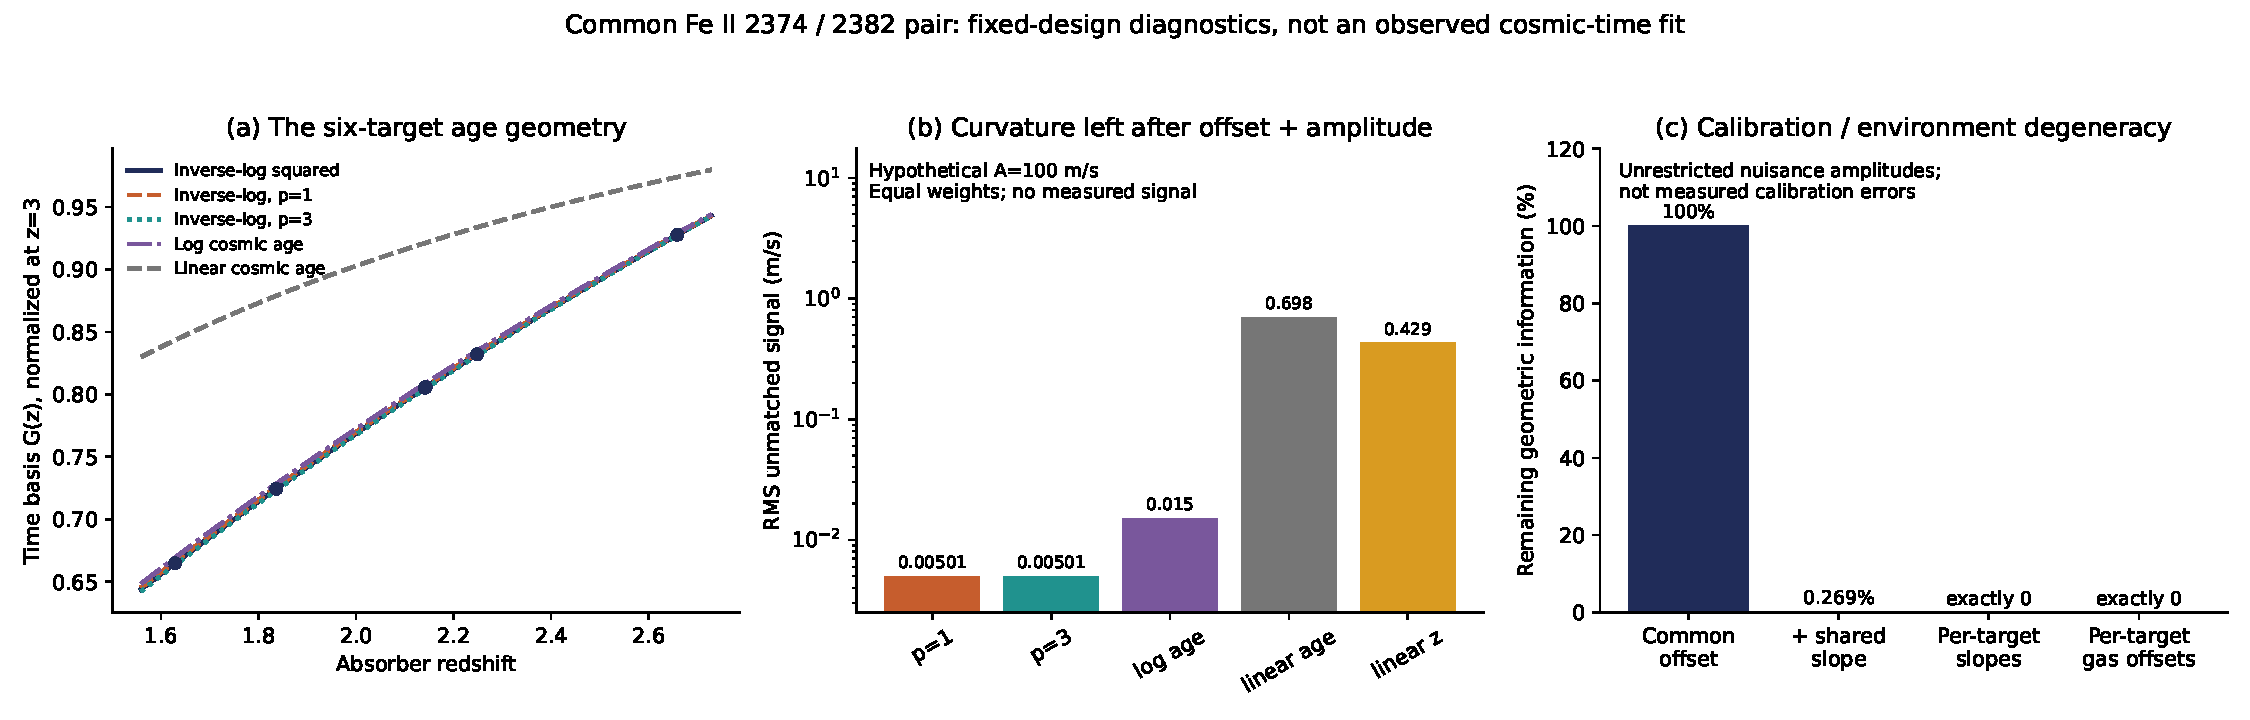
\includegraphics[width=.99\textwidth]{../experiments/highz_feasibility_2026-09-20/results/cross_age/cross_age_identifiability.pdf}
\caption{Fixed-design sensitivity at the six candidate redshifts. The curves and information calculations use no measured line shifts. Free differential offsets for individual absorbers span the age response; more restrictive nuisance assumptions retain conditional information. Competing temporal functions are compared after optimizing their common intercept and amplitude, so raw differences caused only by normalization are removed. All velocity scales in the scenario panels are assumed, not detected.}
\label{fig:age_design}
\end{figure}

The nuisance-space calculation in Fig.~\ref{fig:age_design} illustrates two distinct limitations. Allowing an independently free differential calibration slope for each target gives a full-row-rank nuisance matrix: each slope multiplies a nonzero observed separation of the two transitions. An arbitrary time-amplitude change can then be cancelled exactly. Free target-specific gas or environmental offsets have the same property. This is a statement about identifiability under unrestricted nuisance freedom, not evidence that actual systematics have arbitrary size. A common wavelength zero point cancels between the two lines and cannot produce this degeneracy.

The closeness of this line pair does suppress smooth long-range calibration errors. At the six redshifts its observed separation is approximately $21.83$--$30.38\,\text{\AA}$. Hypothetical velocity-distortion slopes of 50, 200 and $500\,\mathrm{m\,s^{-1}}$ per $1000\,\text{\AA}$ give pair offsets of $1.09$--$1.52$, $4.37$--$6.08$ and $10.92$--$15.19\,\mathrm{m\,s^{-1}}$, respectively. These are propagated scenarios, not adopted empirical priors. If only one slope is shared by all six targets, it leaves $0.269\%$ of the equal-weight age information available with a free intercept alone. However, matching the illustrative $A=100\,\mathrm{m\,s^{-1}}$ age curve actually requires approximately $3077\,\mathrm{m\,s^{-1}}$ per $1000\,\text{\AA}$, with a remaining $0.429\,\mathrm{m\,s^{-1}}$ RMS. Thus a near-degenerate shape cannot be used to claim that modest smooth distortions explain an arbitrarily large effect. Finite independent calibration constraints would restore finite conditional information; short-scale errors and gas-model biases require separate treatment.

Even with those systematics controlled, detecting a trend would not identify its exponent. After re-fitting a common offset and amplitude, $p=1$ and $p=3$ reproduce a $p=2$, $A=100\,\mathrm{m\,s^{-1}}$ scenario to approximately $0.005\,\mathrm{m\,s^{-1}}$ RMS at these six redshifts. An ordinary logarithm of cosmic age differs by $0.015\,\mathrm{m\,s^{-1}}$ RMS, and a linear-age model by $0.698\,\mathrm{m\,s^{-1}}$. These differences arise because a Planck-time reference makes $\ln(t/t_*)$ large compared with its change across this age interval. They scale with the assumed amplitude and are fixed-design model distances, not measured objective differences, detection powers or physical upper bounds.

The pair J053007$-$250329 and J233156$-$090802 is also informative in principle: their rounded catalogue redshifts, 2.141 and 2.143, correspond to an age difference of approximately $2.86\,\mathrm{Myr}$ in this coordinate. The same illustrative age model predicts a difference of only $0.051\,\mathrm{m\,s^{-1}}$. A larger measured difference between such sightlines would test the combined target-dependent effects, provided both descriptors were reliable; it would not uniquely isolate an environmental or instrumental cause. Rounded catalogue redshifts and adopted cosmology do not imply precisely measured ages.

We therefore do not regress the available exploratory offsets into a measured cosmic amplitude. A calibrated cross-age test requires comparable profile constraints, external restrictions on differential systematics, and a specified physical response. The finite set of transitions measures selected energy differences; it does not sample the full symmetry-resolved atomic-level distribution or establish a correspondence to Riemann-zero spacing statistics.

